% Ohne .NET Standard

\section{.NET}

\begin{multicols*}{2}

\subsection{Common Language Runtime}
\begin{itemize}
    \item JIT-Compilers für die Übersetzung von Intermediate Language Code in Maschinencode
    \item Class Loader für das Laden von Klassen-Code zur Laufzeit
    \item Speicherverwaltung mit Garbage Collection
    \item Sprachübergreifendes Debugging
    \item Exceptions
    \item Type Checking und Code Verifikation des IL-Codes
    \item Thread-Verwaltung
    \item COM-Interoperabilität (Interaktion mit unmanaged code)
    \item Basis-Klassen mit System-Funktionen
\end{itemize}
\includegraphics*[width=\columnwidth]{clr}
\subsubsection{Microsoft Intermediate Language - MSIL}
Vorkompilierte Zwischensprache
\begin{itemize}
    \item Prozessor-unabhängig
    \item Assembler-ähnlich
    \item Sprach-unabhängig
\end{itemize}
\subsubsection{JIT}
\begin{itemize}
    \item Normal-JIT: Übersetzt immer das was er gerade braucht.
    \item Pre-JIT: Gesamter Code vor Ausführung z.B. mit NGEN
    \item Econo-JIT: Wie Normal-JIT, aber mit Cleanup-Mechanismus
\end{itemize}
\includegraphics*[width=\columnwidth]{jit}


\subsection{Assemblies}
Kompilation erzeugt Assemblies
\begin{itemize}
    \item Deployment- und Ausführungs-Einheit
    \item Executable (*.exe) oder Library (*.dll)
    \item Dynamisch ladbar
    \item Definiert Typ-Scope
\end{itemize}
\includegraphics*[width=\columnwidth]{assembly}
\subsubsection{Module}
Metadaten beschreiben alle Aspekte des Codes ausser der Programmlogik.
\begin{itemize}
    \item Klassen-Definitionen
    \item Methoden-Definitionen
    \item Feld-Definitionen
\end{itemize}
Metadaten lassen sich über .NET Reflection abfragen.
\nfat{Anwendungen:}
\begin{itemize}
    \item CLR - Verifikation von Typensicherheit
    \item CLR - Memory Management
    \item CLR - JIT Compilation / Erzeugung von Maschinencode
    \item Visual Studio - Object-Browser (Navigation durch System-Assemblies)
    \item Visual Studio - IntelliSense
\end{itemize}

\subsection{Common Type System CTS}
\begin{itemize}
    \item Einheitliche Typen für alle .NET-Programmiersprachen
    \item Typen in Laufzeitsystem definiert, nicht in Sprache
    \item Alle Typen sind von System.Object abgeleitet 
    \item 2 Kategorien von Typen: Reference- und Value-Types
    \item Boxing / Unboxing: Automatische Umwandlung (Value Types – Reference Types)
\end{itemize}
\subsubsection{Reference- \& Value Types}
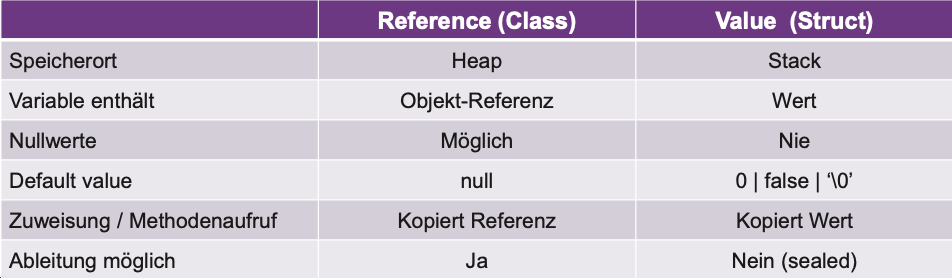
\includegraphics[width=\columnwidth]{refval}
\nfat{Reference:} Garbage Collected, Konstruktor erzeugt \& initialisiert Objekt
\nfat{Value:} Konstruktor macht nur Initialisierung, sealed, Keine Garbage Collection
\\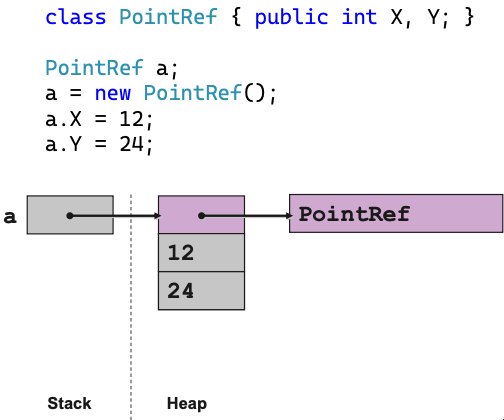
\includegraphics[width=.49\columnwidth]{ref}
\vrule
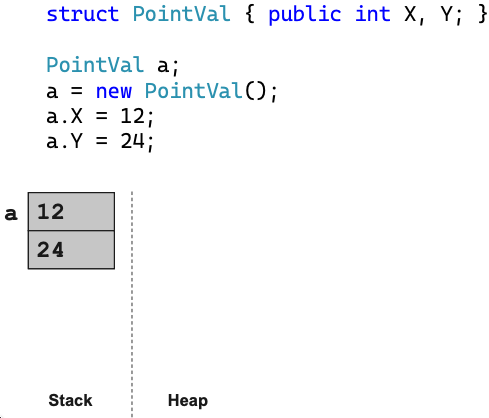
\includegraphics[width=.49\columnwidth]{val}
\fat{Weiteres Beispiel:}
\begin{lstlisting}
public class Person
{
    public int Weight { get; set; }
    public int Height { get; set; }
    public Ethnicity Ethnicity { get; }

    public Person()
    {
        Ethnicity = new();
    }
}

public class Ethnicity
{
    public string Name { get; set; }
}
\end{lstlisting}
\begin{multicols*}{2}
$\uparrow$
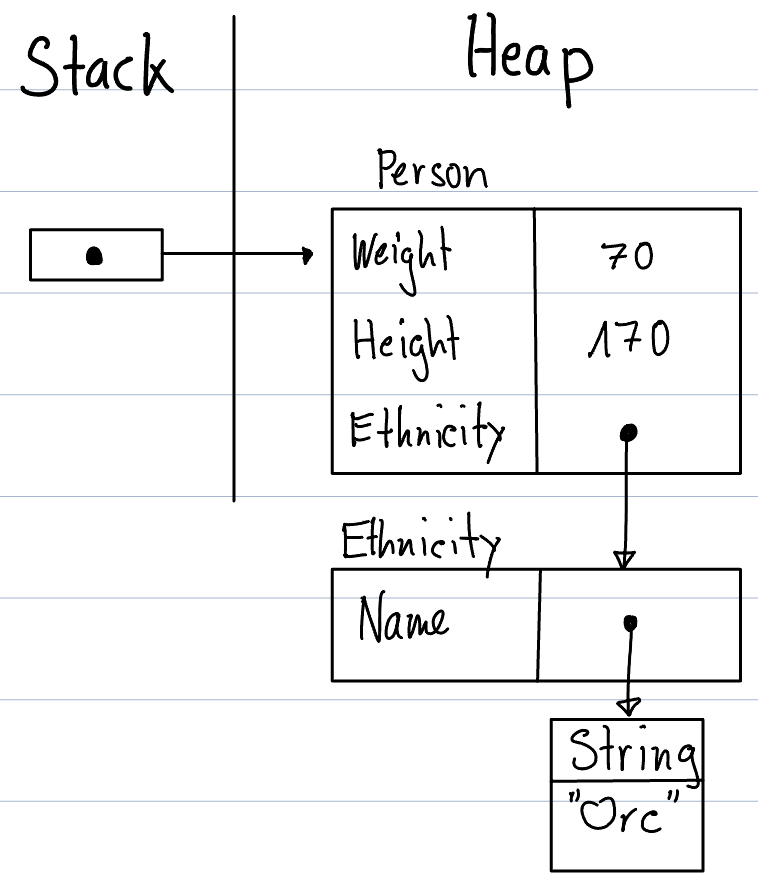
\includegraphics[width=\columnwidth]{stackheap1}
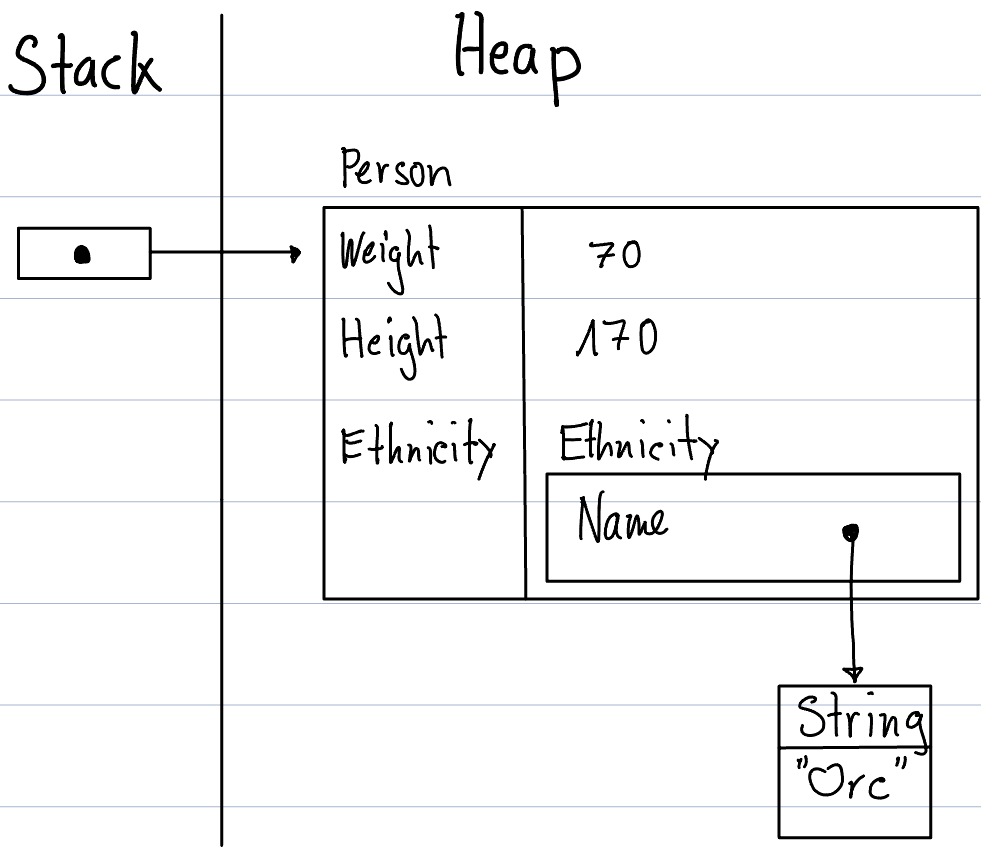
\includegraphics[width=\columnwidth]{stackheap2}
\vfill
$\downarrow$
\end{multicols*}
\begin{lstlisting}
//Änderung zu struct
public struct Ethnicity
{
    public string Name { get; set; }
}
\end{lstlisting}
\subsubsection{Boxing/Unboxing}
\fat{Boxing:} Kopiert Value Type in einen Reference Type, Value Type wird implizit konvertiert: Up Cast
\nfat{Unboxing:} Kopiert Reference Type in einen Value Type, Explizite Konversion nötig: Down Cast / Exceptions möglich!
\\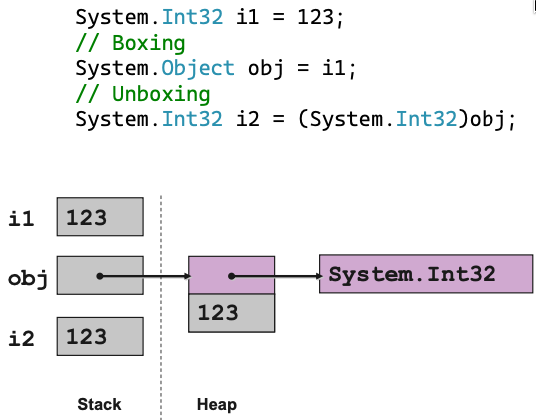
\includegraphics[width=.5\columnwidth]{boxubox}

\subsection{Projektaufbau}
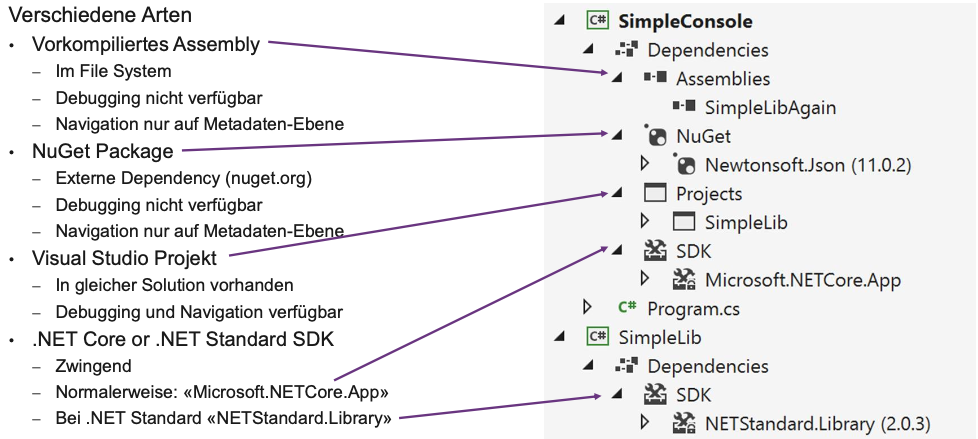
\includegraphics[width=\columnwidth]{projaufbau}
\hrule
\vspace{2mm}
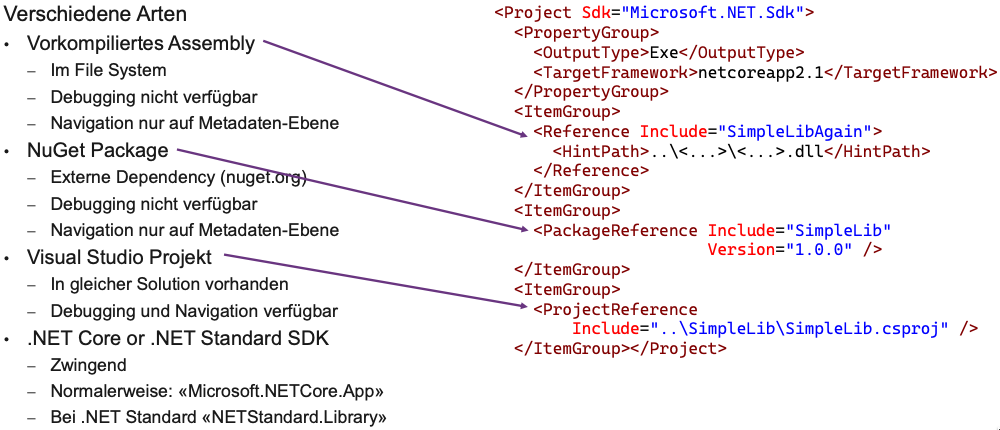
\includegraphics[width=\columnwidth]{projaufbau2}
\subsection{Packages}
\begin{itemize} 
    \item .NET wird neu in kleineren Packages ausgeliefert
    \item Kein monolithisches Framework mehr
    \item Aufgeteilt in verschiedene NuGet Packages, Vorteile:
    \begin{itemize}
        \item Erlaubt unterschiedliche Release-Zyklen
        \item Erhöhte Kompatibilität durch Kapselung OS / CPU spezifischer Komponenten
        \item Kleinere Deployment-Einheiten
    \end{itemize}
\end{itemize}
\subsubsection{Wichtige Packages}
\begin{itemize}
    \item System.Runtime (Wichtigstes Package): Object, String, Array, Action, Func, ...
    \item System.Collections: Generische Listen wie List<T>, Dictionary<TKey,TValue>, ...
    \item System.Net.Http: HttpClient, HttpResponseMessage, ...
    \item System.IO.FileSystem: File, Directory, ...
    \item System.Linq: Enumerable, ILookup<TKey,TElement>, ...
    \item System.Reflection: Assembly, TypeInfo, MethodInfo, ...
\end{itemize}
\subsubsection{NuGet}
NuGet ist der neue Standard für Packaging von Applikationen:
\begin{itemize}
    \item Dateityp: *.nupkg
    \item Inhalt:
    \begin{itemize}
        \item lib Ordner: Libraries (Assemblies), Oft in mehreren .NET Versionen
        \item .nuspec file: Manifest / Metadaten. Beinhalten:
        \begin{itemize}
            \item PackageIdentifier
            \item Titel und Beschreibung
            \item Versions-Information
            \item Dependencies
        \end{itemize}
    \end{itemize}
    \item Als Zip-Datei gespeichert
\end{itemize}
\vspace*{2mm}
\fat{Entwicklungsprozess:}
\begin{itemize}
    \item Create Project (dotnet new)
    \item Create Manifest (*.csproj file)
    \item Compile Project (dotnet build)
    \item Create Package (dotnet pack)
    \item Publish Package (dotnet nuget push)
    \item Consume Package (dotnet add package)
\end{itemize}
\fat{Deployment:}
\begin{itemize}
    \item Lokales NuGet Repository auf Entwicklungsrechner (Local Feed)
    \item Self-hosted NuGet Repository
    \item Hosted NuGet Repository (public / private): NuGet Gallery, Azure DevOps, MyGet, ProGet, etc.
\end{itemize}


\section{C\#}
\subsection{Naming Guideline}
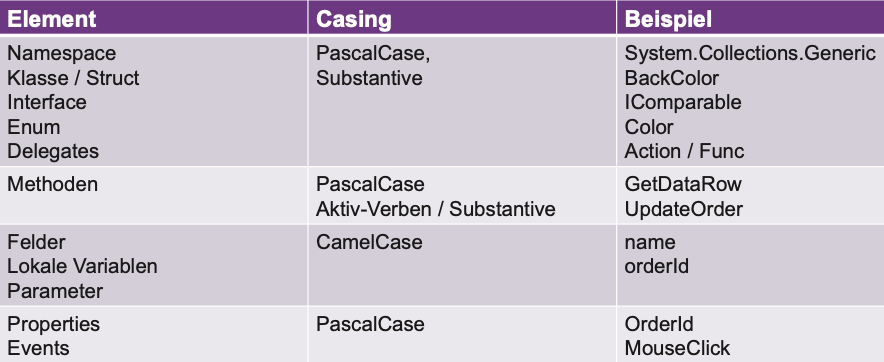
\includegraphics[width=.97\columnwidth]{naming}

\subsection{Sichtbarkeit}
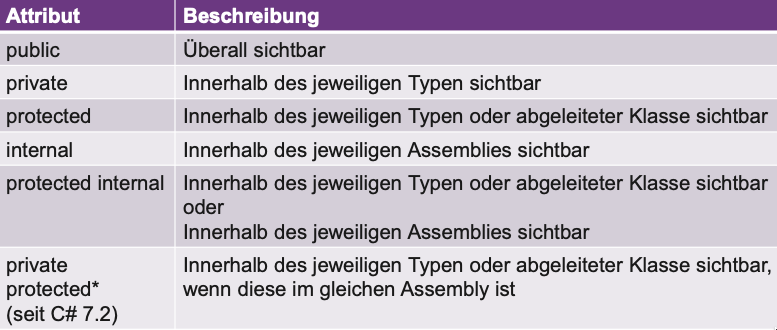
\includegraphics[width=.97\columnwidth]{sichtbarkeit1}
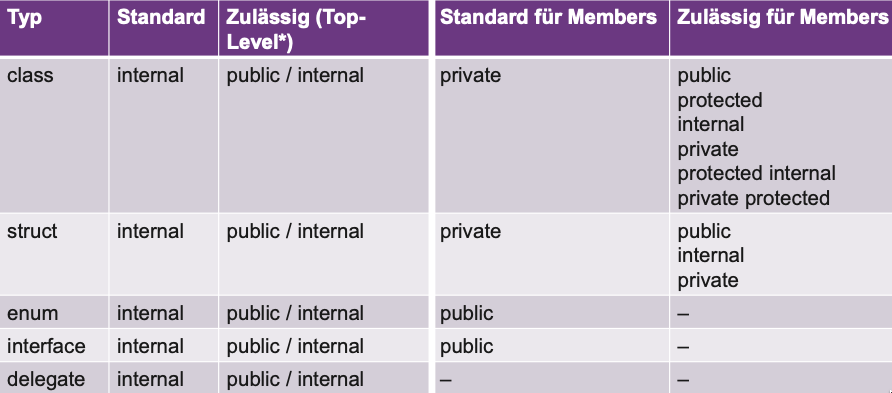
\includegraphics[width=.97\columnwidth]{sichtbarkeit2}

\subsection{Schlüsselwörter}
\includegraphics*[width=.97\columnwidth]{keywords}

\subsection{Primitivtypen (Value)}
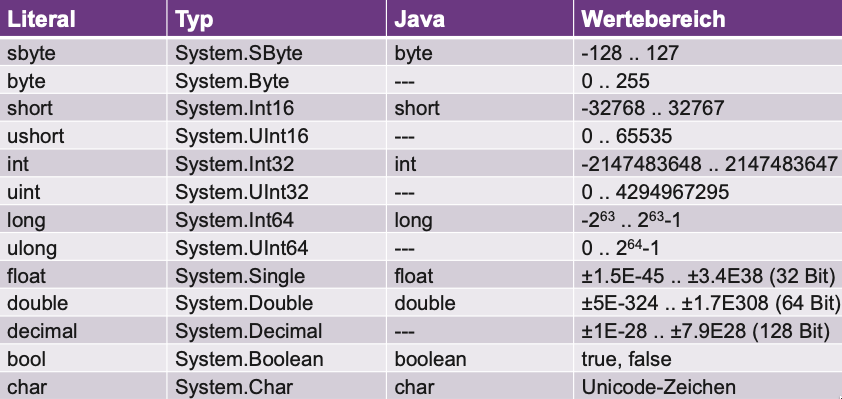
\includegraphics[width=.97\columnwidth]{primitivtypen}\\
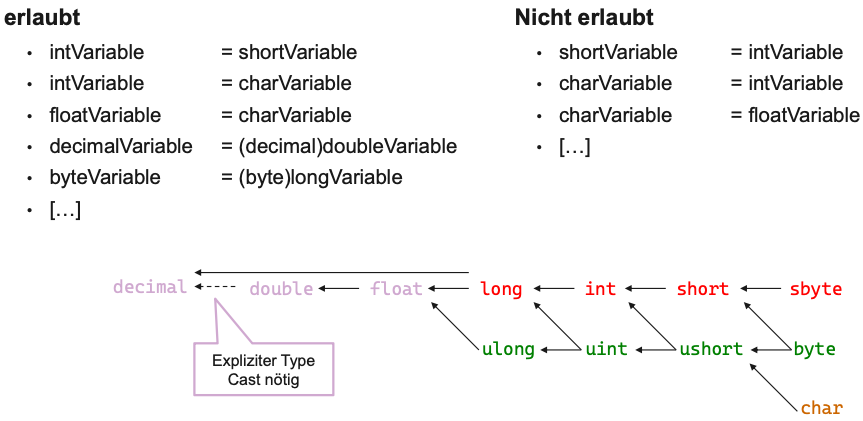
\includegraphics[width=\columnwidth]{casting}
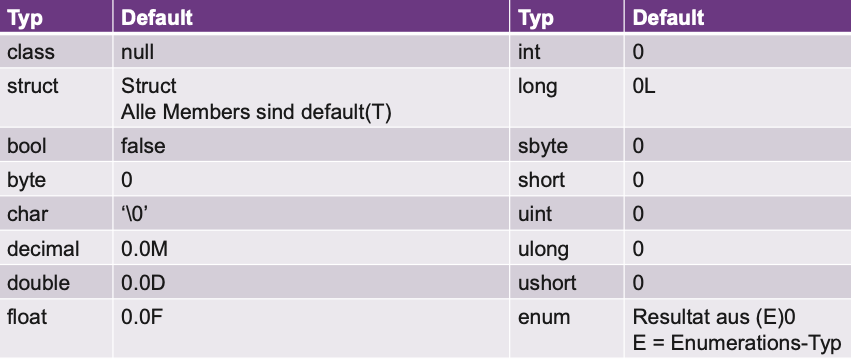
\includegraphics[width=\columnwidth]{default}
\begin{lstlisting}
int x = default(int);
int x = default; // C# 7.1
\end{lstlisting}

\subsection{Operatoren}
\fat{Rangfolge:}
\includegraphics*[width=\columnwidth]{rangfolge1}
\includegraphics*[width=\columnwidth]{rangfolge2}

\subsubsection{Arithmetische}
Erlaubte Operanden: Numerische, Chars, Enums
\\Resultat: Kleinstmöglicher numerischer Typ, minimum int
\subsubsection{Vergleich}
Erlaubte Operanden für ==, != : Alle Datentypen
\\Erlaubte Operanden für $<,>,<=,>=$ : Numerische, Chars, Enums
\\x is T : x = Ausdruck mit beliebigem Datentyp, T = Beliebiger Datentypname
\begin{lstlisting}
if (1 == 2) { /* ... */ }
if ("a" == "a") { /* ... */ }
if (1 != 2) { /* ... */ }
bool b1 = 2.0 > 1.0;
bool b2 = 2.0 < 1.0;
bool b3 = 'a' >= 'a';
bool b4 = 'a' <= 'b';
bool b5 = "a" <= "b"; // Compilerfehler
if ("a" is object) { /* ... */ } bool b6 = 1 is bool;
bool b7 = "a" is string;
\end{lstlisting}
\subsubsection{Logische}
Erlaubte Operanden für $||, \&\&$: bool
\\Resultat: bool
\\short-circuit Evaluation, stoppt sobald Resultat eindeutig. 
\\Bei $\&\&$ wenn linker Teil false ist
\\Bei $||$ wenn linker Teil true ist
\begin{lstlisting}
bool b1 = false && false; // false 
bool b2 = true && false; // false 
bool b5 = false || false; // false 
bool b6 = true || false; // true 
bool b8 = true || true; // true
if (true && false) { /* ... */ }
if ("a" == "b" || false) { /* ... */ } 
\end{lstlisting}
\subsubsection{Overflow}
\begin{lstlisting}
int y = checked(x * x);

checked
{
    int z = x * x
}
\end{lstlisting}
\subsubsection{typeof / sizeof}
\fat{typeof}
\begin{lstlisting}
// System.Int32
Type t1 = typeof(int);
// System.Object
Type t2 = typeof (object);
// System.Int32
Type t3 = 123.GetType();
\end{lstlisting}
\fat{sizeof}
\begin{itemize}
    \item Liefert die Datengrösse in Bytes
    \item Funktioniert nur mit Value Types
    \item Auf Structs zwingend in unsafe Block
\end{itemize}
\begin{lstlisting}
Console.WriteLine(sizeof(int)); 
Console.WriteLine(sizeof(MyEnum)); 
unsafe
{
    Console.WriteLine(sizeof(MyStruct)); 
}
\end{lstlisting}
\subsection{Statements}
\subsubsection{switch}
\begin{lstlisting}
string ctry = "Germany"; 
string language; 
switch (ctry)
{
    case "England":
    case "USA":
        language = "English";
        break;
    case "Germany":
    case "Austria":
    case "Switzerland":
        language = "German";
        break; 
    case null:
        Console.WriteLine("Coutry null");
        break;
    default:
        Console.WriteLine("Unknown " + ctry);
        break; 
}
\end{lstlisting}

\subsection{Namespaces}
\begin{itemize}
    \item Mehrere Namespaces in einem File möglich
    \item Namespace und Ordnerstruktur können sich unterscheiden
\end{itemize}
\begin{lstlisting}
using System; //Import Namespace

namespace A
{   // gilt nur in dieser Datei für A
    using C; 
}
namespace B { using D; }

using F = System.Windows.Forms; //Alias
\end{lstlisting}
\subsubsection{File-scoped Namespaces}
\begin{lstlisting}
// File1.cs Klassisch
namespace OstDemo
{
    classX{}
}
// File1.cs File-scoped Namespace ab C# 10
namespace OstDemo;
class X { }
namespace OstDemo2 { } // Compiler-Fehler
\end{lstlisting}
\subsubsection{Global Usings}
Gelten für das ganze Projekt.
\nfat{Deklaration:}
\begin{itemize}
    \item In Datei GlobalUsings.cs: using static Azure.Core;
    \item MSBuild / *.csproj Datei: <ItemGroup><Using Include=\dq Azure.Core\dq /></ItemGroup>
\end{itemize}
\fat{Implizite Usings:} <ImplicitUsings>enable</ImplicitUsings> im *.csproj
\subsubsection{Statische Usings}
\begin{itemize}
    \item Nur statische Klassen sowie Enums erlaubt
    \item Importiert alle statischen Members, statischen Nested Types
\end{itemize}
\begin{lstlisting}
using static System.Console; 
using static System.Math; 
using static System.DayOfWeek;

class ExamplesStaticUsing
{
    static void Test() 
    {
        WriteLine(Sqrt(3 * 3 + 4 * 4));
        WriteLine(Friday - Monday);
    } 
}
\end{lstlisting}

\subsection{Main-Methode}
Zwingend für Executables (Console Application, Windows Application, etc.)
\begin{lstlisting}
// Examples
static void Main() { }
static int Main() { }
static void Main(string[] args) { }
static int Main(string[] args) { }
static async Task Main() { }
static async Task<int> Main() { }
static async Task Main(string[] args) { }
static async Task<int> Main(string[] args) { }
\end{lstlisting}

\subsection{Enumerationstypen}
Liste von Konstanten inklusive Wert (Default-Typ Int32)
\begin{lstlisting}
//Leitet implizit von Int32 ab, beginn bei 0
enum Days { Sun, Mon, Tue, Wed, Thu, Fri, Sat };
int sunValue = (int)Days.Sun;
// Ausgabe: Sunday / #0
Console.WriteLine("{0} / #{1}.", Days.Sun, sunValue); 

//Beginn bei 10, Sun & Sat = 10 -> ist ok
enum Days { Sun = 10, Mon, Tue, Wed, Thu, Fri = 9, Sat };
enum Days : byte { Sun, Mon, Tue, Wed, Thu, Fri, Sat };
byte today = (byte)Days.Monday; //Verwendung

//String zu Enum
//Non-Generic (Exception on failure)
Days day1 = (Days)Enum.Parse(typeof(Days), "Mon"); 
//Generic
Days day2;
bool success2 = Enum.TryParse("Mon", out day2);
//Generic / C# 7.0
bool success3 = Enum.TryParse("Mon", out Days day3); 

//Ausgabe
foreach (string name in Enum.GetNames(typeof(Days))) 
{
    Console.WriteLine(name);
}
\end{lstlisting}

\subsection{Arrays}
\begin{itemize}
    \item Referenztyp $\rightarrow$ Immer auf dem Heap
    \item Länge aller Dimensionen bei Instanzierung bekannt
    \item Alle Werte sind nach Instanzierung initialisiert (false, 0, null, etc.)
\end{itemize}
\subsubsection{Eindimensional}
\begin{lstlisting}
int[] a1 = new int[5]; //Deklaration (Value Type)
int[] a2 = new int[] { 1, 2 }; //Deklaration & Definition
int[] a3 = int[] { 1, 2 }; //Ohne new
int[] a4 = { 1, 2 }; // Ohne new / Typ
object[] a5 = new object[5]; //Deklaration (Ref Type)

int[] a3 = { 1, 2, 3, 4, 5, 6 }; 
a3 = new int[] {1,2,3,4,5,6}; 
a3 = new [] { 1, 2, 3, 4, 5, 6 };

int length = a1.Length;
\end{lstlisting}
\subsubsection{Mehrdimensional rechteckig}
\begin{lstlisting}
int[,] multiDim1 = new int[2, 3]; //Deklaration
int[,] multiDim2 = {{1,2,3},{4,5,6}}; //Wertedefinition

int[,] a1 = new int[3,2];
int len = a1.Length; //Liefert 6
int len0 = a1.GetLength(0); //Liefert 3 (0. Dimension)
int len1 = a1.GetLength(1); //Liefert 2 (1. Dimension)
\end{lstlisting}
\subsubsection{Mehrdimensional jagged}
\begin{lstlisting}
int[][] jaggedA = new int[6][]; //Deklaration
jaggedA[0] = new int[] { 1, 2, 3, 4 }; //Wertdefinition

int[][] a1 = new int[2][]; 
a1[0] = new int[3]; 
a1[1] = new int[1];
int len = a1.Length; //Liefert 2 (0. Dimension)
int len0 = a1[0].Length; //3
int len1 = a1[1].Length; //1
\end{lstlisting}
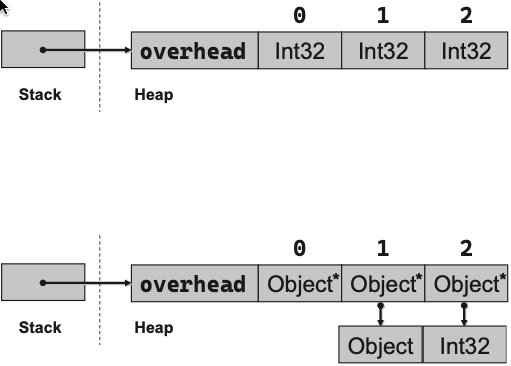
\includegraphics[width=.49\columnwidth]{1arr}
\vrule
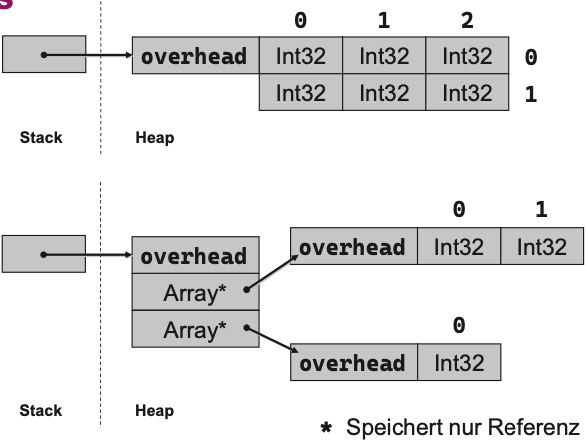
\includegraphics[width=.49\columnwidth]{marr}
\fat{Vorteile Blockmatrizen:}
\begin{itemize}
    \item Verbraucht weniger Speicher, da weniger Referenzen verwaltet werden müssen.
    \item Speicher kann als gesamter Block alloziert werden.
    \item Bei Jagged Arrays sind Dimension 2-n manuell zu allozieren.
    \item Schnellere Garbage Collection
\end{itemize}

\subsection{Strings}
\begin{itemize}
    \item Klasse / Reference Type
    \item string ist ein Alias für System.String
    \item Nicht modifizierbar
    \item Wertevergleich mit == Operator / Equals-Methode möglich
    \item Nicht mit $\backslash$0 terminiert
    \item Länge wird durch Property «Length» ermittelt
    \item Verkettung mit +
\end{itemize}
\subsubsection{Interpolation}
\begin{lstlisting}
string s3 = $"{DateTime.Now}: {"Hello"}";
string s4 = $"{DateTime.Now}: {(DateTime.Now.Hour < 18 ? "Hello" : "Good Evening")}";  
\end{lstlisting}
\subsubsection{Vergleiche}
\begin{lstlisting}
string s1 = "Test"; 
string s2 = "Test"; 
string s3 = "Not Test";
//True
bool result1 = s1.Equals(s2);
bool result2 = string.Equals(s1, s2);
bool result3 = s1 == s2;
//False
bool result4 = s1.Equals(s3);
bool result5 = string.Equals(s1, s3);
bool result6 = s1 == s3;
\end{lstlisting}
\subsubsection{Interning}
Strings werden intern wiederverwendet
Erst string.Copy(...) erzeugt eine echte Kopie

\begin{lstlisting}
string s1 = "Test"; 
string s2 = "Test";
bool result1 = string.Equals(s1, s2);
bool result2 = string.ReferenceEquals(s1, s2); // True

string s3 = string.Copy(s1);
bool result3 = string.Equals(s1, s3); // True 
bool result4 = string.ReferenceEquals(s1, s3); // False
\end{lstlisting}
\end{multicols*}